\documentclass[conference]{IEEEtran}
\IEEEoverridecommandlockouts
\usepackage{amsmath,amssymb,amsfonts}
\usepackage{algorithmic}
\usepackage{graphicx}
\usepackage{textcomp}
\usepackage{xcolor}
\def\BibTeX{{\rm B\kern-.05em{\sc i\kern-.025em b}\kern-.08em
    T\kern-.1667em\lower.7ex\hbox{E}\kern-.125emX}}
\begin{document}

%\title{How Safe is C to Rust Translation Using LLMs}
\title{How Safe is C to Rust Translation Using LLMs?}

\author{
\IEEEauthorblockN{Kenneth Fulton}
\IEEEauthorblockA{\textit{Dept. of CEMS} \\
\textit{Texas A\&M University - San Antonio}\\
San Antonio, US \\
kfult01@jaguar.tamu.edu}
\and
\IEEEauthorblockN{Joshua Ibrom}
\IEEEauthorblockA{\textit{Dept. of CEMS} \\
\textit{Texas A\&M University - San Antonio}\\
San Antonio, US \\
jibro01@jaguar.tamu.edu}
}

\maketitle

\begin{abstract}
The increasing adoption of Rust has prompted efforts to rewrite insecure C codebases, traditionally used for low-level applications, into safer Rust equivalents. While manual C-to-Rust translation is labor-intensive and
error-prone, Large Language Models (LLMs) offer a promising automated alternative, as explored in
initiatives like DARPA’s TRanslating All C TO Rust (TRACTOR) project \cite{darpa_c_to_rust}. This study investigates
the safety and reliability of LLM-based C-to-Rust translation, focusing on ChatGPT’s ability to
handle C code with memory safety errors. Results reveal persistent challenges, including missing crate dependencies, runtime panics from memory or index errors, and warnings for unused imports or
deprecated methods. Despite adding common crates to mitigate dependency issues, LLM translation
succeeded in less than half of small programs, aligning with prior findings that only 11\% of C
pointers convert to safe Rust references \cite{emre2023aliasing}. These outcomes emphasize the need for hybrid approaches
combining other C to Rust conversion tools and manual refinement to achieve safe Rust code.
\end{abstract}

\begin{IEEEkeywords}
programming language translation, ai safety
\end{IEEEkeywords}

\section{Background}
Traditional systems-level programming of embedded software, operating systems,
and other low-level applications has been done with language such as C so that
memory and other system components may be managed by the programmer as needed.
With this form of programming also comes the potential for pitfalls that leave
applications ``open to exploits, crashes, or corruption'' 
\cite{klabnik2018rust_book}. With the increasing popularity of Rust, a
systems-level programming language promising safety from the common C / C++
pitfalls, there is now the question of how we might perform some re-write of
critical system software from their potentially insecure C versions to ones
written in Rust \cite{klabnik2018rust_book, emre2021translating}.

One such method of performing a re-write of some codebase is to attempt to
hand-roll a new version of that software by manually translating line-by-line
given C code to Rust code---a method that is time consuming, expensive, and
may lead to there being missing or incorrectly-implemented blocks of code.
Another such approach that has now become far more feasible with the
prevalence and advanced reasoning abilities of \textit{large language models}
(LLMs) is to use those LLMs to perform automatic translation with human
verification.

\subsection{Research Questions}
\begin{enumerate}
    \item How reliably can LLMs resolve memory safety errors when converting 
        C code to Rust?
    \item How efficiently can LLMs translate C code to Rust?
    \item How can you prove that Rust code is safe?
\end{enumerate}


\section{Related Work}
Rust's rich type system and ownership model guarantee memory and thread safety, delivering high-performance applications with reduced risks of exploits, crashes, or corruption. Leveraging these benefits, the Defense Advanced Research Projects Agency (DARPA) has initiated the TRanslating All C TO Rust (TRACTOR) project, using Large Language Models (LLMs) to convert C codebases into Rust, aiming to produce secure, high-quality Rust code matching the expertise of skilled Rust developers \cite{darpa_c_to_rust}. However, translating unsafe C code to safe Rust remains challenging, as static analysis struggles to convert most C pointers to safe Rust references (only \(\sim\)11\%) and LLM-based auto-translation succeeds in less than half of small C programs as found by Li et al. \cite{li2024translating}, necessitating advanced techniques like static analysis, LLM repair, and manual intervention to preserve C code properties in well-typed Rust programs \cite{eniser2024towards}. Some common C-to-Rust conversion tools include C2Rust for transpilation, LLMs for experimental translation, Rust Analyzer for refactoring and of course manual rewriting. Each approach alone faces challenges like pointer aliasing and limited automation, but hybrid strategies may help achieve safe, idiomatic Rust code. In this study, we evaluate the performance of ChatGPT, a widely used LLM for C-to-Rust conversion, focusing on its ability to handle C code containing memory safety issues.


\section{Proposed Approach}
In this experiment, we created C code with memory errors and collected samples from a GitHub dataset \cite{thakur2025beginners}. A Python script was used to translate each \texttt{.c} file into Rust using two prompting strategies: the first instructed the LLM to ``Convert the following C code to Rust, providing only the complete Rust code in plaintext,'' (hereinafter referred to as the \textit{Simple Prompt}) while the second added ``while preserving all memory safety errors, if feasible'' (hereinafter referred to as the \textit{Unsafe Prompt}). The resulting \texttt{.rs} files were stored in an outputs directory, and a testing Python script executed each Rust file, recording whether it ran successfully, encountered compilation errors, or produced runtime errors (See Figure \ref{fig:Figure 1}).
\begin{figure}
    \centering
    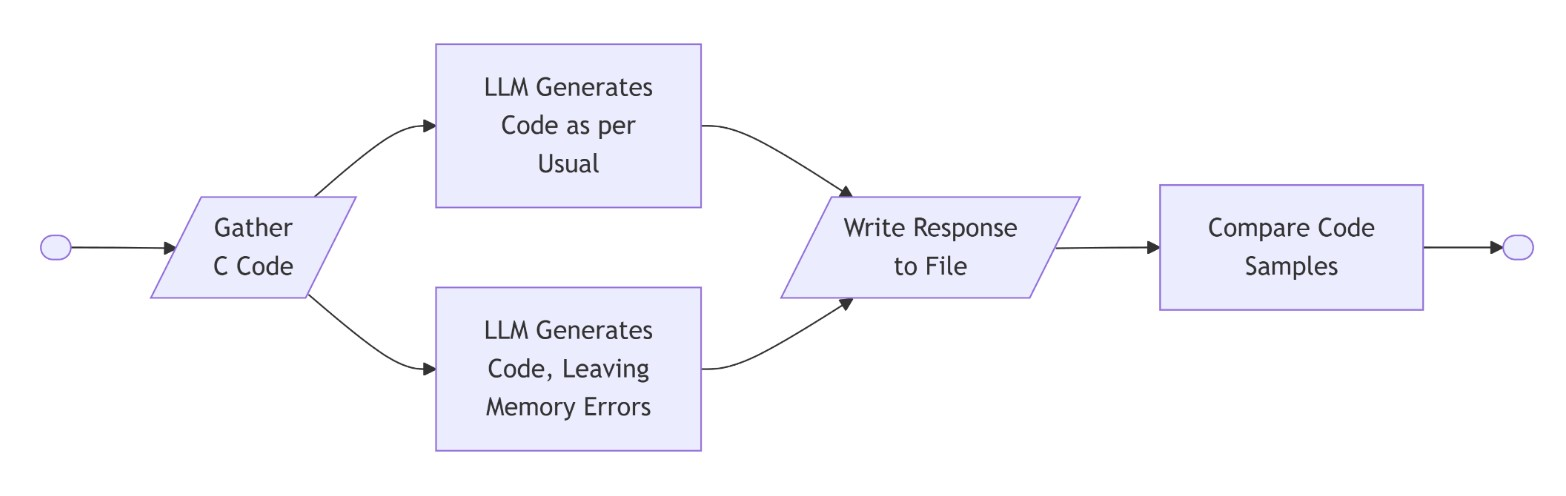
\includegraphics[width=1.0\linewidth]{Experimental Approach.jpg}
    \caption{Experimental Approach}
    \label{fig:Figure 1}
\end{figure}


\section{Experimentation}

-+
\section{Experiment Outcomes and Observations}

\begin{figure}
    \centering
    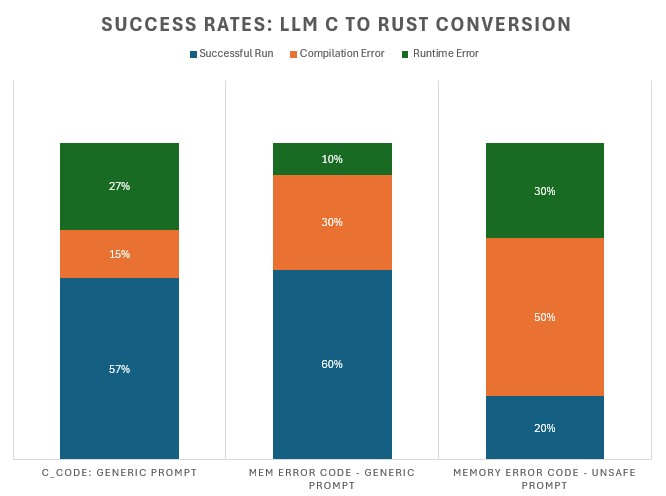
\includegraphics[width=1.0\linewidth]{Success Rates.jpg}
    \caption{Rust Execution Success Rates}
    \label{fig:enter-label}
\end{figure}

Several recurring issues were observed during the C-to-Rust conversion process. Common problems included mismatched types, particularly in function arguments and return values, as well as missing dependencies, where files attempted to use crates such as \texttt{libc}, \texttt{chrono}, and \texttt{users} without proper linkage or inclusion in the \texttt{Cargo.toml} file. This was circumvented in part by adding a list of common crates to the \texttt{Cargo.toml} file referenced by the python testing script. These included \texttt{serde}, \texttt{tokio}, \texttt{anyhow}, \texttt{thiserror}, \texttt{lazy\_static}, \texttt{log}, \texttt{once\_cell}, \texttt{rayon}, \texttt{derive\_builder}, \texttt{libc}, \texttt{users} and \texttt{chrono}. Additionally, runtime panics frequently occurred due to memory-related errors, index out-of-bounds violations, or thread-related issues. Furthermore, many generated Rust files triggered warnings related to unused imports, unused variables, or the use of deprecated methods.

In some instances, such as Rust code samples which were generated using the Unsafe Prompt, these errors were to be expected. For
example, the code shown


\section{Conclusion}

\bibliographystyle{IEEEtran}
\bibliography{paper/sources}
\end{document}